%!TEX root = ../LaTeX-cn.tex
\chapter{\LaTeX\ 进阶}

本章的内容多数与宏包的使用相关.记得使用texdoc命令查看宏包的使用手册,这是学习宏包最好的手段,没有之一.

\section{自定义命令与环境}
\label{sec:newcommand}
自定义命令是\LaTeX\ 相比于字处理软件MS Word之流最强大的功能之一.它可以大幅度优化你的文档体积,用法是:
\begin{latex}
\newcommand{`\textit{cmd}`}[`\textit{args}`][`\textit{default}`]{`\textit{def}`}
\end{latex}

现在来解释一下各个参数:
\begin{para}
\item[cmd:] 新定义的命令,不能与现有命令重名.
\item[args:] 参数个数.
\item[default:] 首个参数,即\texttt{\#{}1}的默认值.你可以定义只有一个参数、且参数含默认值的命令.
\item[def:] 具体的定义内容.参数1以\texttt{\#{}1}代替,参数2以\texttt{\#{}2}代替,以此类推.
\end{para}

如果重定义一个现有命令,使用\latexline{renewcommand}命令,用法与\latexline{newcommand}一致.简单的例子:
\begin{latex}
% 加粗:\concept{text}
\newcommand{\concept}[1]{\textbf{#1}}
% 加粗#2并把#1#2加入索引,默认#1为空.
% 比如\cop{Sys}或者\cop[Sec.]{Sys}
\newcommand{\cop}[2][]{\textbf{#2}}\index{#1 #2}}
\end{latex}

如果想定义一个用于数学环境的命令,借助\latexline{ensuremath}命令.它保证其参数会在数学模式下运转, 且即使已位于数学模式中也不会报错.
\begin{latex}
\renewcommand\qedsymbol{\ensuremath{\Box}}
\end{latex}

自定义环境的命令是\latexline{newenvironment},也可以定义多个参数.注意后段定义中不能使用参数,但你可以“先保存后调用”.例子:
\begin{latex}
\newenvironment{QuoteEnv}[2][]
    {\newcommand\Qauthor{#1}\newcommand\Qref{#2}}
    {\medskip\begin{flushright}\small ——~\Qauthor\\
    \emph{\Qref}\end{flushright}}
\end{latex}

下面是效果:
\begin{codeshow}
\begin{QuoteEnv}[William Butler]{When you are old}
But one man loved the pilgrim soul in you.
And loved the sorrows of your changing face.
\end{QuoteEnv}
\end{codeshow}

\section{箱子:排版的基础}
\label{sec:box}

\begin{wrapfigure}{R}{0.4\textwidth}
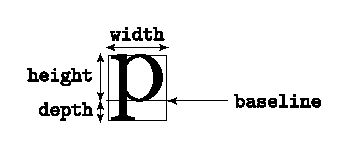
\includegraphics{Texcharbox.pdf}
\caption{箱子的参数}
\label{fig:boxpara}
\end{wrapfigure}

\LaTeX\ 排版的基础单位就是“箱子(box)”,例如整个页面是一个矩形的箱子,侧边栏、主正文区、页眉页脚也都是箱子.在正常排版中,文字应当位于箱子内部;如果单行文字过长、没能正确断行,造成文字超出箱子,这便是Overfull的坏箱(bad box);如果内容太少,导致文字不能美观地填满箱子,便是Underfull的坏箱.

如\fref{fig:boxpara}所示,箱子的三个参数:高度(height)、宽度(width)和深度(depth).分隔高度和深度的是基线.

\subsection{无框箱子}
命令\latexline{mbox}产生一个无框的箱子,宽度自适应.有时用它来强制“结合”一系列命令,使之不在中间断行.比如\TeX\ 这个命令的定义(其中\latexline{raisebox}命令在后面介绍):
\begin{latex}
\mbox{T\hspace{-0.1667em}\raisebox{-0.5ex}{E}\hspace{-0.125em}X}
\end{latex}

或者也可以使用命令\latexline{makebox[width][pos]\{text\}},宽度由width参数指定.pos参数的取值可以是l, s, r即居左、两端对齐、居右,还有竖直方向的t, b两个参数.

无框小页的使用方法是\texttt{minipage}环境,参数类似\latexline{parbox}:
\begin{latex}
\begin{minipage}[pos]{width}
\end{latex}

\subsection{加框箱子}
命令\latexline{fbox}产生加框的箱子,宽度自动调整,但不能跨行.命令\latexline{framebox}类似上面介绍的\latexline{makebox}.如果是想在数学环境下完成加框,使用\latexline{boxed}命令.

width参数中,可以用\latexline{width}, \latexline{height}, \latexline{depth}, \latexline{totalheight}分别表示箱子的自然宽度、自然高度、自然深度和自然高深度之和.

\begin{codeshow}
\fbox{This is a frame box} \\
\framebox[2\width]{double-width}\\
\begin{equation}\boxed{x^2=4}
\end{equation}
\end{codeshow}

加宽盒子的宽度、以及内容到盒子的距离可以自行定义.默认定义是:
\begin{latex}
\setlength{\fboxrule}{0.4pt} \setlength{\fboxsep}{3pt}
\end{latex}

加框小页使用\envi{boxedminipage}环境(需要\pkg{boxedminipage}宏包).

\subsection{竖直升降的箱子}
命令\latexline{raisebox}可以把文字提升或降低,它有两个参数:

\begin{codeshow}
A\raisebox{-0.5ex}{n} example.
\end{codeshow}

\subsection{段落箱子}
段落箱子的强大之处在于它提供自动换行的功能,当然你需要指定宽度.
\begin{latex}
\parbox[pos]{width}{text}
\end{latex}

以及例子:

\begin{codeshow}
This is \parbox[t]{3.5em}{an long
example to show} how \parbox[b]
{4em}{`parbox' works perfectly}.
\end{codeshow}

\subsection{缩放箱子}
宏包\pkg{graphicx}提供了一种可缩放的箱子\latexline{scalebox\{h-sc\}[v-sc]\{pbj\}},注意其中水平缩放因子是必要参数.缩放内容可以是文字也可以是图片,例子:
\begin{codeshow}
\LaTeX---\scalebox{-1}[1]{\LaTeX}\\
\LaTeX---\scalebox{1}[-1]{\LaTeX}\\
\LaTeX---\scalebox{-1}{\LaTeX}\\
\LaTeX---\scalebox{2}[1]{\LaTeX}
\end{codeshow}

此外还有\latexline{resizebox\{width\}\{heigh\}\{text\}}命令.

\subsection{标尺箱子}
命令\latexline{rule[lift]\{width\}\{height\}}能够画出一个黑色的矩形.你可以在单元格中使用width, height其一为0的该命令,作一个隐形的“支撑”来限定单元格的宽或高.而\latexline{strut}命令则用当前字号大小设置高度与深度.例如:

\begin{codeshow}
\begin{tabular}{|c|}
  \hline
  \rule[-1em]{1em}{1ex}text
  \rule{0pt}{38pt} \\
  \hline
  2nd text\strut--- \\
  \hline
\end{tabular}
\end{codeshow}

\subsection{覆盖箱子}
有时候需要把一段文字覆盖到另一段上面,使用\latexline{llap}或\latexline{rlap}.什么?你从没这么干过?但或许有一天你需要呢?

\begin{codeshow}
你看不清这些字\llap{是什么}\\
\rlap{这些}你也看不清
\end{codeshow}

\subsection{旋转箱子}
宏包\pkg{graphicx}提供了\latexline{rotatebox}命令,参数与插图命令相同.
\begin{codeshow}
\rotatebox[origin=c]{90}{专}治颈椎病.
\end{codeshow}

\subsection{颜色箱子}
\label{subsec:colorbox}
\pkg{xcolor}宏包支持的颜色箱子命令有:

\begin{codeshow}
\textcolor{red}{红色}强调\\
\colorbox[gray]{0.95}{浅灰色背景} \\
\fcolorbox{blue}{cyan}{%
\textcolor{blue}{蓝色边框+文字,
  青色背景}}
\end{codeshow}

命令\latexline{fcolorbox}可以调整\latexline{fboxrule, \char`\\fboxsep}参数,而\latexline{colorbox}只能调整后者.参考前面的加框箱子一节.

强大的\pkg{tcolorbox}宏包专门定义了众多的箱子命令,参考\secref{subsec:tcolorbox}.

\section{复杂距离}
\label{sec:hvspace}
\subsection{水平和竖直距离}
长度单位参考\hyperref[sec:length]{这里}介绍过的内容.水平距离命令有两种,一种禁止在此处断行,如\tref{tab:nobreak-hspace};另一种允许换行,如\tref{tab:break-hspace}.
\begin{table}[!htb]
\centering
\caption{禁止换行的水平距离}
\label{tab:nobreak-hspace}
\begin{tabular}{p{12em}p{8em}p{6em}}
  \latexline{thinspace}或\latexline{,} & 0.1667em & \rule{8pt}{2pt}\thinspace\rule[4pt]{8pt}{2pt} \\
  \latexline{negthinspace}或\latexline{!} & -0.1667em & \rule{8pt}{2pt}\negthinspace\rule[4pt]{8pt}{2pt} \\
  \latexline{enspace} & 0.5em & \rule{8pt}{2pt}\enspace\rule[4pt]{8pt}{2pt} \\
  \latexline{nobreakspace}或\char`~{} & 空格 & \rule{8pt}{2pt}\nobreakspace\rule[4pt]{8pt}{2pt}
\end{tabular}
\end{table}

\begin{table}[!htb]
\centering
\caption{允许换行的水平距离}
\label{tab:break-hspace}
\begin{tabular}{p{12em}p{8em}p{6em}}
  \latexline{quad}          & 1em           & \rule{8pt}{2pt}\quad\rule[4pt]{8pt}{2pt} \\
  \latexline{qquad}         & 2em           & \rule{8pt}{2pt}\qquad\rule[4pt]{8pt}{2pt} \\
  \latexline{enskip}        & 0.5em         & \rule{8pt}{2pt}\enskip\rule[4pt]{8pt}{2pt} \\
  \latexline{\textvisiblespace} & 空格 & \rule{8pt}{2pt}\ \rule[4pt]{8pt}{2pt}
\end{tabular}
\end{table}

使用\latexline{hspace\{length\}}命令自定义空格的长度,其中\textit{length}的取值例如:\texttt{-1em, 2ex, 5pt plus 3pt minus 1pt, 0.5\char92{}linewidth}等.如果想要这个命令在断行处也正常输出空格,使用带星命令\latexline{hspace*}.

类似地使用\latexline{vspace}和\latexline{vspace*}命令,作为竖直距离的输出.

要定义新的长度宏,使用\latexline{newlength}命令;要重设现有长度宏的值,可以选择使用\latexline{setlength}命令;要调整长度宏的值,则使用\latexline{addtolength}命令.
\begin{latex}
\newlength{\mylatexlength}
\setlength{\mylatexlength}{10pt}
\addtolength{\mylatexlength}{-5pt}
\end{latex}

此外,\LaTeX\ 还定义了三个竖直长度\latexline{smallskip}, \latexline{medskip}, 和\latexline{bigskip}:

\begin{codeshow}
\parbox[t]{3em}{TeX\par TeX}
\parbox[t]{3em}{TeX\par\smallskip TeX}
\parbox[t]{3em}{TeX\par\medskip TeX}
\parbox[t]{3em}{TeX\par\bigskip TeX}
\end{codeshow}

\subsection{填充距离与弹性距离}
命令\latexline{fill}用于填充距离,需要作为\latexline{hspace}或\latexline{vspace}的参数使用.另外还有单独使用的命令\latexline{hfill}与\latexline{vfill},作用相同.

弹性距离指以一定比例计算得到的多个空白,命令是\latexline{stretch}.例子:

\begin{codeshow}
Left\hspace{\fill}Right\\
Left\hspace{\stretch{1}}Center
\hspace{\stretch{2}}Right
\end{codeshow}

你还可以使用类似\latexline{hfill}的\latexline{hrulefill}和\latexline{dotfill}命令:

\begin{codeshow}
L\hfill R\\
L\hrulefill Mid\dotfill R
\end{codeshow}

\subsection{行距}
\LaTeX\ 的行距由基线计算,可以使用命令\latexline{linespread\{num\}},默认的基线距离\latexline{baselineskip}是1.2倍的文字高.所以默认行距是1.2倍;如果更改linespread为1.3,那么行距变为$1.2\times 1.3=1.56$倍——这也是ctex文档类的做法.

此外还有\latexline{lineskiplimit}和\latexline{lineskip}命令.有时候在两行之间,可能包含较高的内容(比如分式$\dfrac{1}{2}$),使得前一行底部与后一行顶部的距离小于limit值,则此时行距会从由\latexline{linespread}改为由\latexline{lineskip}控制.本手册采用:
\begin{latex}
\setlength{\lineskiplimit}{3pt}
\setlength{\lineskip}{3pt}
\end{latex}

\subsection{制表位*}
制表位使用\envi{tabbing}环境,需要指出,这是一个极其容易造成坏箱的环境.几个要点:
\begin{para}
\item[\char92{}=] 在此处插入制表位.
\item[\char92{}>] 跳入下一个制表位.
\item[\char92{}\char92{}] 制表环境内必须手动换行和缩进.
\item[\char92{}kill] 若行末用\verb|\kill|代替\verb|\\|,那么该行并不会被实际输出到文档中.
\end{para}

一个丑陋的例子:
\begin{codeshow}[listing and text]
\begin{tabbing}
\hspace{4em}\=\hspace{8em}\=\kill
制表位 \> 就是这样 \> 使用的 \\
随时 \> 可以添加 \> 新的: \= 就这样 \\
也可以 \= 随时重设 \= 制表位 \\
这是 \> 新的 \> 一行
\end{tabbing}
\end{codeshow}

\subsection{悬挂缩进*}
这种缩进在实际排版中并不常用,经常是列表需要的场合才使用,但那可以借助列表宏包\pkg{enumitem}进行定义.这里介绍的是正文中的悬挂缩进使用.

如果需要对单独一段进行悬挂缩进,例如使用:
\begin{latex}
\hangafter 2
\hangindent 6em
\end{latex}

\hangafter 2
\hangindent 6em
这两行放在某一段的上方,作用是控制紧随其后的段落从第2行开始悬挂缩进,并且设置悬挂缩进的长度是\texttt{6em}.

如果需要对连续的多段进行悬挂缩进,可以改造编号列表环境或者\envi{verse}环境\footnote{事实上这是一个排版诗歌的环境,参考前文的\hyperref[envi:verse]{这里}.}来实现.或者尝试:

\begin{codeshow}
正文...

{\leftskip=3em\parindent=-1em
\indent 这是第一段.注意整体需要放在
一组花括号内,且花括号前应当有空白行
.第一段前需要加indent命令,最后一段
的末尾需额外空一行,否则可能出现异常.

这是第二段.

\ldots

这是最后一段.别忘了空行.

}
\end{codeshow}

\subsection{整段缩进*}
宏包\pkg{changepage}提供了一个\envi{adjustwidth}环境,它能够控制段落两侧到文本区(而不是页边)两侧的距离.
\begin{latex}
\begin{adjustwidth}{1cm}{3cm}
本段首行缩进需要额外手工输入.本环境距文本区左侧1cm,右侧3cm.
\end{adjustwidth}
\end{latex}

也可以尝试赋值\latexline{leftskip}等命令,对奇偶页处理更有效.

\section{自定义章节样式}
\label{sec:titlesec}
这一节主要涉及\pkg{titlesec}宏包的使用.章节样式调整使用\latexline{titlelabel},\latexline{titleformat*}命令.前者需要配合计数器使用,后者简单地设置章节标题的字体样式.例如:
\begin{latex}
\titlelabel{\thetitle.\quad}
\titleformat*{\section}{\itshape}
\end{latex}

章节样式由标签和标题文字两部分构成.标签一般表明了大纲级别以及编号,比如“第一章”、“Section 3.1”等.标题文字比如“自定义章节样式”这几个字.还记得吗?在report与book类的subsection及以下,article类的paragraph及以下是默认没有编号的.因此对应的级别也没有标签,除非人工进行设置.

对于需要详细处理标签、标题文字两部分的情况,\pkg{titlesec}宏包还提供了一个\latexline{titleformat}命令.调用方式:
\begin{latex}
\titleformat{`\itshape command`}[`\itshape shape`]{`\itshape format`}{`\itshape label`}{`\itshape sep`}
    {`\itshape before-code`}[`\itshape after-code`]
\end{latex}

它们对应的含义如下:
\begin{para}
\item[command:] 大纲级别命令,如\latexline{chapter}等.
\item[shape:] 章节的预定义样式,分为9种:
  \begin{para}
  \item[hang] 缺省值.标题在右侧,紧跟在标签后.
  \item[block] 标题和标签封装排版,不允许额外的格式控制.
  \item[display] 标题另起一段,位于标签的下方.
  \item[runin] 标题与标签同行,且正文从标题右侧开始.
  \item[leftmargin] 标题和标签分段,且位于左页边.
  \item[rightmargin] 仿上.右页边.
  \item[drop] 文本包围标题.
  \item[wrap] 类似drop,文本会自动调整以适应最长的一行.
  \item[frame] 类似display,但有框线.
  \end{para}
\item[format:] 用于设置标签和标题文字的字体样式.这里可以包含竖直空距,即标题文字到正文的距离.
\item[label:] 用于设置标签的样式,比如“第\latexline{chinese\char`\\thechapter}章”大概是ctexbook类的默认样式设置.
\item[sep:] 标签和标题文字的水平间距,必须是\LaTeX\ 的长度表达.当shape取display时,表示竖直空距;取frame时表示标题到文本框的距离.
\item[before:] 标题前的内容.
\item[after:] 标题后的内容.对于hang, block, display,此内容取竖向;对于runin, leftmargin, 此内容取横向;否则此内容被忽略.
\end{para}

宏包还给出了\latexline{titlespacing}与\latexline{titlespacing*}两个命令.使用方式是:
\begin{latex}
\titlespacing*{`\itshape command`}{`\itshape left`}{`\itshape before-sep`}{`\itshape after-sep`}[`\itshape right-sep`]
\titlespacing{`\itshape command`}{`\itshape left`}{`\itshape *m`}{`\itshape *n`}[`\itshape right-sep`]
\end{latex}

各参数的含义:
\begin{para}
\item[command:] 大纲级别命令,如\latexline{chapter}
\item[label:] 缩进值.在left/right margin下表示标题宽;在wrap中表示最大宽;在runin中表示标题前缩进的空距.
\item[before-sep:] 标题前的垂直空距.
\item[after-sep:] 标题与正文之间的空距.hang, block, display中是垂直空距;runin, wrap, drop, left/right margin中是水平空距.
\item[right-sep:] 可选.仅对hang, block, display适用.
\item[*m/*n:] 在\latexline{titlespacing}命令中的\textit{m, n}分别表示before与after sep的变动范围倍数,基数是默认值.
\end{para}

宏包中还有一个 \latexline{titleclass} 命令,用来定义新的章节命令(例如 \verb|\subchapter|)或者重申明已有的章节命令:
\begin{latex}
% 使 \part 命令不单独占据一页
\titleclass{\part}{top}
% 新定义一个 \subchapter 命令
\titleclass{\subchapter}{straight}[\chapter]
\newcounter{subchapter}
\renewcommand{\thesubchapter}{\Alph{subchapter}}
\end{latex}
其中,第二参数表示章节类型,可以是 \texttt{page}(独占一页),\texttt{top}(另开新页),或者 \texttt{straight}(普通).

最后,宏包还给出了\latexline{titleline}命令,用来绘制填充整行、同时又嵌有其他对象的行.对象可以嵌入到左中右lcr三个位置.如果你只是想填充一行而不嵌入对象,使用\latexline{titlerule}及其带星号的命令形式.
\begin{latex}
% 嵌入对象的线
\titleline[c]{CHAPTER 1}
% 单纯填充一行
\titlerule[`\itshape height`]
\titlerule*[`\itshape width`]{`\itshape text`}
\end{latex}

最后,给出本手册中的样式定义,作为例子.这个例子稍微有些复杂,只使用到了\latexline{titleformat}相关的命令.
\begin{latex}
\newcommand{\chaformat}[1]{%
    \parbox[b]{.5\textwidth}{\hfill\bfseries #1}%
    \quad\rule[-12pt]{2pt}{70pt}\quad
    {\fontsize{60}{60}\selectfont\thechapter}}
% chapter样式定义中的\chaformat以章名作为隐式参数
\titleformat{\chapter}[block]{\hfill\LARGE\sffamily}
    {}{0pt}{\chaformat}[\vspace{2.5pc}\normalsize
    \startcontents\printcontents{}{1}
    {\setcounter{tocdepth}{2}}]
\titleformat*{\section}{\centering\Large\bfseries}
\titleformat{\subsubsection}[hang]
    {\bfseries\large}{\rule{1.5ex}{1.5ex}}{0.5em}{}
\end{latex}

本例没有定义subsection样式.如果你想给subsection级别标号(即赋予它标签),使用:\latexline{setcounter\{secnumdepth\}\{3\}}\footnote{report/book类part级别深度为0,递增;article类part为-1,无chapter级别.故section及以下深度一致.}.

临时更改\latexline{secnumdepth}可以生成不编号的章节,但章节名仍会被使用在目录和\latexline{markboth}中——有时这比带星号的章节命令更巧妙一些.

\section{自定义目录样式}
\label{sec:titletoc}
这一节主要涉及\pkg{titletoc}宏包,它与\pkg{titlesec}宏包的文档写在同一个pdf中.上节的例子(即本手册Chapter)涉及\latexline{startcontents}与\latexline{printcontents}命令,旨在每一章的开始插入本章的一个目录.

首先是目录的标题,可以通过renewcommand更改.分别是 \latexline{contentsname}, \latexline{listfigurename}, \latexline{listtablename}三个.

再来看命令\latexline{dottecontents}与命令\latexline{titlecontents}:
\begin{latex}
\dottecontents{`\itshape section`}[`\itshape left`]{`\itshape above-code`}
    {`\itshape label-width`}{`\itshape leader-width`}
\titlecontents{`\itshape section`}[`\itshape left`]{`\itshape above-code`}{`\itshape numbered-entry-format`}
    {`\itshape numberless-entry-format`}{`\itshape filler-page-format`}[`\itshape below-code`]
\end{latex}

各参数的含义:
\begin{para}
\item[section:] 目录对象.可以填chapter, section, 或者figure, table.
\item[left:] 目录对象左侧到左页边区的距离.请作必选使用.
\item[above-code:] 格式调整命令.可以包含垂直对象,也可以用\latexline{contentslabel},即指定本级别目录标签箱子的宽度.
\item[label-width:] 标签宽.
\item[leader-width:] 填充符号宽.默认的填充符号是圆点.
\item[numered-entry-format:] 如果有标签,则在目录文本前输入的格式.
\item[numberless-entry-format:] 如果没有标签输入的格式.
\item[filler-page-format:] 填充格式.一般借助\pkg{titlesec}中的\latexline{titlerule*}命令.
\item[below-code:] 在entry之后输入的格式,比如垂直空距.
\end{para}

本手册目录样式定义,其中section级别使用了填充命令\latexline{titlerule*}:
\begin{latex}
\titlecontents{chapter}[1.5em]{}{\contentslabel{1.5em}}
    {\hspace*{-2em}}{\hfill\contentspage}
\titlecontents{section}[3.3em]{}
    {\contentslabel{1.8em}}{\hspace*{-2.3em}}
    {\titlerule*[8pt]{$\cdot$}\contentspage}
\titlecontents*{subsection}[2.5em]{\small}
    {\thecontentslabel{}}{}
    {, \thecontentspage}[;\qquad][.]
\end{latex}

\section{自定义图表}
\label{sec:figtab}
\subsection{长表格}
包括\pkg{supertabular}, \pkg{longtable}, \pkg{tabu}在内的多个宏包都能完成长表格的排版,大致的功能会包括:
\begin{para}
\item[表头控制:] 首页的表头样式,以及转页后表头的样式.
\item[转页样式:] 在表格跨页时,页面最下方插入的特殊行,比如to be continued.
\end{para}

这里主要介绍\pkg{longtable}宏包.主要命令:
\begin{para}
\item[\latexline{endhead}] 定义每页顶端的表头.在表头行用该命令代替\latexline{\char`\\\char`\\}命令来换行即可.
\item[\latexline{endfirsthead}] 如果首页的表头与其他页不同,使用该命令.
\item[\latexline{endfoot}] 定义每页底端的表尾.
\item[\latexline{endlastfoot}] 另外定义末页底端的表尾.
\item[\latexline{caption}] 与原生tabular的该命令一致.如果你不想显示表格编号,使用带星的该命令;如果不想让其加入表格目录,在可选参数中留空\latexline{caption[]\{...\}}.
\item[\latexline{label}] 注意\verb|\label|命令不能被用在多页对象中,请在表体中或者firsthead/lastfoot中使用.
\item[\latexline{LTleft}] 表格左侧到主文本区边缘的距离,默认是\latexline{fill}.你可以用:

\latexline{setlength\char`\\LTleft\{0pt\}}来取消这个距离,进行居左.
\item[\latexline{LTright}] 类似.
\item[\latexline{LTpre}] 表格上部到文本的距离,默认是\latexline{bigskipamount}\footnote{这个命令通常是一行左右的竖直距离,12pt$\pm$4pt左右.}.
\item[\latexline{LTpost}] 类似.
\item[\latexline{\char`\\ \char91\ldots\char93}] 在换行后插入竖直空距.
\item[\latexline{\char`\\{*}}] 禁止在该行后立刻进行分页.
\item[\latexline{kill}] 该行不显示,但用于计算宽度.
\item[\latexline{footnote(mark/text)}] 命令\latexline{footnote}不能用于表头或表尾;在表头和表尾中,使用\latexline{footnotemark}命令,并在表外用\latexline{footnotetext}写明脚注内容.
\end{para}

\pkg{longtable}宏包支持的表格可选参数是clr,不能使用t或b. 此外,\RED{longtable中的跨列可能需要编译多次才能正常显示.}最后给出一个例子:

\begin{longtable}{@{*}r||p{3cm}@{*}}
KILLED & LINE! \kill

\caption[\texttt{longtable} Example]{This is an example}\\
\hline
\multicolumn{2}{@{}c@{}}{This is the headfirst\footnotemark}\\
First Col & Second Col \\
\hline\hline
\endfirsthead

\caption*{--Continued Longtable--}\\
\hline\hline
\multicolumn{2}{@{}c@{}}{This is the head of other page}\\
First Here & Second Here \\
\hline
\endhead

\hline\hline
This is the & bottom. \\
\hline
\endfoot

\hline
\textbf{That's all} & \textbf{and thanks}. \\
\hline
\endlastfoot

\footnotetext{Footnotemark: first footnote in table head.}
This is an example & and you can \\
see how longtable will & work. \\
Space after line are & allowed. \\[25ex]
You can adjust LTright and & LTleft \\
if you want to. I'd like & to set \\
LTleft as ``0pt'', but it all & depends on\\
you. And maybe you can try & footnote \\
like this\footnote{Footnote example.} and also
& footnotetext\footnotemark\footnotetext{Footnotetext example.}. \\
As for footnotemark, you've seen it & in the firsthead.\\[15ex]
And I think maybe it's long & enough to make \\
a table across pages, so go to the & next page and \\
check whether the head at next page is & different from \\
that on this page. Also you can have a look & at lastfoot. \\[20ex]
So do you get how to use this & package? \\
Maybe you'll love it. So enjoy & \texttt{longtable}!
\end{longtable}

它的代码如下:
\begin{latex}
\begin{longtable}{@{*}r||p{3cm}@{*}}
KILLED & LINE! \kill

\caption[\texttt{longtable} Example]{This is an example}\\
\hline
\multicolumn{2}{@{}c@{}}{This is the headfirst\footnotemark}\\
First Col & Second Col \\
\hline\hline
\endfirsthead

\caption*{--Continued Longtable--}\\
\hline\hline
\multicolumn{2}{@{}c@{}}{This is the head of other page}\\
First Here & Second Here \\
\hline
\endhead

\hline\hline
This is the & bottom. \\
\hline
\endfoot

\hline
\textbf{That's all} & \textbf{and thanks}. \\
\hline
\endlastfoot

\footnotetext{Footnotemark: first footnote in table head.}
This is an example & and you can \\
see how longtable will & work. \\
Space after line are & allowed. \\[25ex]
You can adjust LTright and & LTleft \\
if you want to. I'd like & to set \\
LTleft as ``0pt'', but it all & depends on\\
you. And maybe you can try & footnote \\
like this\footnote{Footnote example.} and also
& footnotetext\footnotemark
\footnotetext{Footnotetext example.}. \\
As for footnotemark, you've seen it & in the firsthead.\\[15ex]
And I think maybe it's long & enough to make \\
a table across pages, so go to the & next page and \\
check whether the head at next page is & different from \\
that on this page. Also you can have a look & at lastfoot.
\\[20ex]
So do you get how to use this & package? \\
Maybe you'll love it. So enjoy & \texttt{longtable}!
\end{longtable}
\end{latex}

\subsection{\texttt{booktabs}:三线表}
\pkg{booktabs}宏包提供\latexline{toprule}, \latexline{midrule}与\latexline{bottomrule}命令来绘制三线表.更多需要的横线可以通过\latexline{midrule}添加.
\begin{codeshow}
\begin{tabular}{cccc}
\toprule
& \multicolumn{3}{c}{Numbers} \\
\cmidrule{2-4}
& 1 & 2 & 3 \\
\midrule
Alphabet & A & B & C \\
Roman & I & II& III \\
\bottomrule
\end{tabular}
\end{codeshow}

命令\latexline{cmidrule}如果连续使用,还能写成\latexline{cmiderule(lr)}的形式,使其向内缩进一小段,造成相互“断开”的样子.\dpar

\subsection{彩色表格}
彩色表格依靠\pkg{colortbl}宏包,它会调用\pkg{array}和\pkg{color}宏包.但是可以在加载\pkg{xcolor}宏包时添加table选项来调用\pkg{colortbl}宏包.

首先是命令\latexline{columncolor},给表格某列加背景色.其中mode参数是指rgb/cmyk等.left/right-ex参数表示向两侧填充的距离,默认是\latexline{tablecolsep}.
\begin{latex}
\columncolor[mode]{colorname}[left-ex][right-ex]
\end{latex}

命令\latexline{rowcolor}和\latexline{cellcolor}分别用于更改表头行的颜色和单个单元格的颜色,放置在表格内对应位置即可.在\pkg{xcolor}支持下还可以使用\latexline{rowcolors}命令,但放在表格开始之前:
\begin{latex}
% 表线为单横,从第2行开始,奇数行绿,偶数行青
\rowcolors[\hline]{2}{green}{cyan}
\begin{tabular}...
\end{latex}

要临时开关奇偶行颜色,使用\latexline{show/hide rowcolors}命令.

彩色表格中跨行,需要把跨行命令放在最后一行,并跨负数行:
\begin{codeshow}
\rowcolors{2}{green}{cyan}
\begin{tabular}{ll}
\hline Col 1 & Col 2\\
& A\\ \multirow{-2}*{Hey} & B\\
\hline
\end{tabular}
\end{codeshow}

\subsection{子图表}
子图表输出用\pkg{subcaption}宏包,它需要与\pkg{caption}宏包共同加载.比如:
\begin{latex}
\usepackage{caption,subcaption}
  \captionsetup[sub]{labelformat=simple}
  \renewcommand{\thesubtable}{(\alph{subtable})}
% 用\ref引用得到如“图1.1(a)”的效果
\begin{table}
\caption{Parents}
\begin{subtable}[b]{0.5\linewidth}
  \centering
  \begin{tabular}{|c|c|}
  A & B \\ \end{tabular}
  \caption{First}\label{...}
\end{subtable}  
\begin{subtable}[b]{0.5\linewidth}
  \centering
  \begin{tabular}{|c|c|}
  A & B \\ C & D \end{tabular}
  \caption{Second}
\end{subtable}  
\end{table}
\end{latex}

效果如\tref{subtab:subcaption1}与\tref{subtab:subcaption2}.更多的请参考\pkg{caption}宏包.
\begin{table}[!htb]
\caption{Parents}
\begin{subtable}[b]{0.5\linewidth}
  \centering
  \begin{tabular}{|c|c|}
  A & B \\ \end{tabular}
  \caption{First}\label{subtab:subcaption1}
\end{subtable}  
\begin{subtable}[b]{0.5\linewidth}
  \centering
  \begin{tabular}{|c|c|}
  A & B \\ C & D \end{tabular}
  \caption{Second}\label{subtab:subcaption2}
\end{subtable}  
\end{table}

\subsection{GIF 动态图}
使用 \pkg{animate} 宏包(当然,\pkg{graphicx} 宏包也是需要的),可以将多张图片以动态图的形式插入 PDF.需要注意的是,\textbf{动态图在一些功能较弱的 PDF 浏览器中可能无法正常工作},推荐使用 Adobe 系列 PDF 浏览器以保证正常浏览.代码如下:
\begin{latex}
\begin{figure}[!hbt]
  \centering
  \animategraphics[controls, autoplay, loop,
  width=0.6\linewidth]{20}{Py3-matplotlib-}{0}{98}
\end{figure}
\end{latex}

以上代码对应的动态图\footnote{该例由 Python - matplotlib 绘制.可以参考\href{https://wklchris.github.io/Py3-matplotlib.html}{此页面}的附录.}给出如\fref{fig:GIF}所示:
\begin{figure}[!hbt]
  \centering
  \animategraphics[controls, autoplay, loop, width=0.6\linewidth]{20}{Py3-matplotlib-}{0}{98}
  \caption{动态图示例}\label{fig:GIF}
\end{figure}

以上会搜索文件夹(包括你在 \pkg{graphicx} 中设置的文件夹),找到图片依次序编号的从“Py3-matplotlib-0.png”到“Py3-matplotlib-98.png”的这99张图片,以每秒20帧为默认播放速度加载.参数 \texttt{controls} 表示在图片下方附加控制按钮,可以暂停/播放,正放/倒放,手动浏览帧,以及更改播放速度.参数 \texttt{autoplay} 表示当阅读者浏览到动态图所在页面时,动态图会自动开始播放.参数 \texttt{loop} 表示播放到尾帧后自动重播.最后,你可以像一般图片加载一样,指定它的 \texttt{width/height}.

注意:如果你只有GIF图像,但安装了\href{https://www.imagemagick.org/script/download.php}{ImageMagick},可以在图像文件夹下使用命令行命令:

\begin{verbatim}
convert Py3-matplotlib.gif -coalesce Py3-matplotlib.png
\end{verbatim}

来将单个 GIF 转为符合上述要求的多个 png 图像.

\section{自定义编号列表}
\label{sec:list}
编号列表的自定义主要使用\pkg{enumitem}宏包.主要的计数器有:
\begin{feai}
\item enumerate:
  \begin{feai}
    \item \textbf{Counter:} enumi, enumii, enumiii, enumiv
    \item \textbf{Label:} labelenumi, labelenumii, \ldots
  \end{feai}
\item itemize: 只有Label,该列表没有Counter. 
  \begin{feai}
    \item \textbf{Label:} labelitemi, labelitemii, \ldots
  \end{feai}
\item description: 只有\latexline{descriptionlabel}定义,默认:
\begin{latex}
\newcommand*{\descriptionlabel}[1]{\hspace\labelsep
    \normalfont\bfseries #1} % \labelsep标签间距,默认0.5em
\end{latex}
\end{feai}

列表\envi{enumerate}, \envi{itemize}的默认参数见\tref{tab:enumitemdes}.

\begin{table}[!hbt]
\centering
\caption{编号列表默认参数表}
\label{tab:enumitemdes}
\renewcommand{\arraystretch}{0.9}
\begin{tabular}{@{}c@{\,}c*{2}{>{\small}l@{}>{\ttfamily\char`\\}l}@{}}
\hline
环境 & 层 & Label & \multicolumn{1}{l}{默认} & Counter & \multicolumn{1}{l}{默认}	\\
\hline
\multirow{4}*{\envi{enumerate}} & 1 & \latexline{labelenumi} & theenumi. & \latexline{theenumi} & arabic\{enumi\}\\
& 2 & \latexline{labelenumi} & (theenumii) & \latexline{theenumii} & alph\{enumi\} \\
& 3 & \latexline{labelenumiii} & theenumiii. & \latexline{theenumiii} & roman\{enumi\} \\
& 4 & \latexline{labelenumiv} & theenumiv. & \latexline{theenumiv} & Alph\{enumiv\} \\
\hline
\multirow{4}*{\envi{itemsize}} & 1 & \latexline{labelitemi} & \multicolumn{3}{p{.5\textwidth}}{\ttfamily\char`\\ textbullet \dotfill\fbox{\textbullet}} \\
& 2 & \latexline{labelitemii} & \multicolumn{3}{p{.5\textwidth}}{\ttfamily\char`\\ textendash \dotfill\fbox{\textendash}}  \\
& 3 & \latexline{labelitemiii} & \multicolumn{3}{p{.5\textwidth}}{\ttfamily\char`\\ textasteriskcentered \dotfill\fbox{\textasteriskcentered}} \\
& 4 & \latexline{labelitemiv} & \multicolumn{3}{p{.5\textwidth}}{\ttfamily\char`\\ textperiodcentered \dotfill\fbox{\textperiodcentered}} \\
\hline
\end{tabular}
\end{table}

在\envi{enumerate}列表中,编号样式按照:1.$\rightarrow$(a)$\rightarrow$i.$\rightarrow$A的顺序嵌套,分别代表\latexline{theenumi}, \latexline{theenumii}, \latexline{theenumiii}, \latexline{theenumiv}的值.你可以通过计数器命令来指定编号样式,不过要额外加上一个星号,比如\latexline{arabic*}表示阿拉伯数字.一个例子:
\begin{codeshow}
\begin{enumerate}\item First
  \begin{enumerate}\item Second
     \begin{enumerate}\item Third
       \begin{enumerate}
       \item Fourth Layer
\end{enumerate}\end{enumerate}
\end{enumerate}\end{enumerate}
% 改为首层小写罗马数字,放于圆括号
\renewcommand{\theenumi}
  {\roman{enumi}}
\renewcommand{\labelenumi}
  {(\theenumi)}
\begin{enumerate}
\item First-layer symbol has changed!
\end{enumerate}
\end{codeshow}

你也可以在\pkg{ctex}宏包被调用(包括ctex文档类被使用)时,在导言区加入:
\begin{latex}
\AddEnumerateCounter{\chinese}{\chinese}{}
\end{latex}

这样就可以将汉字指定为编号样式了.

宏包\pkg{enumitem}可添加参数于列表后,像\verb|\begin{list}[options]|:
\begin{para}
\item[label] 定义\envi{enumerate}环境的编号样式,或者\envi{itemize}环境的符号样式.
\item[ref] 设置嵌套序号格式,比如\texttt{[ref=\char`\\emph\{\char`\\alph*\}]}表示引用的上层序号是强调后的小写字母.你也可以写:\texttt{[label=\char`\\alph\{enumi\}.\ \char`\\roman*]}.
\item[label*] 加在\envi{enumerate}上层序号上.比如上层是2,那么就是2.1, 2.1.1……
\item[font/format] 设置label的字体.如果环境是description, 那么就会设置\latexline{item}命令后方括号内的文本字体.
\item[align] 对齐方式默认right, 也可以选择left/parleft.
\item[start] 初始序号.start=2表示初始序号是2, b, B, ii或II.
\item[resume] 不需赋值的布尔参数.表示接着上一个\envi{enumerate}环境的结尾进行编号.
\item[resume*] 不需赋值的布尔参数.表示完全继承上一个\envi{enumerate}环境的参数.如果你常常使用这个命令,也许你可以新定义一个列表环境.
\item[series] 给当前列表起名(比如mylist),可以在后文中用\texttt{resume=mylist}进行继续编号.
\item[style] 定义\envi{description}列表的样式.
\begin{para}
\item[standard:] label放在盒子中.
\item[unboxed:] label不放在盒子中,避免异常长度或空格.
\item[nextline:] 如果label过长,text会另起一行.
\item[sameline:] 无论label多长,text从label同一行开始.
\item[multiline:] label会被放在一个宽为leftmargin的parbox中.
\end{para}
\end{para}

在列表定义中可能碰到的参数如\fref{fig:enumitemsep}.其中加粗加斜的\LaTeX\ 不原生支持.
\begin{figure}[!hbt]
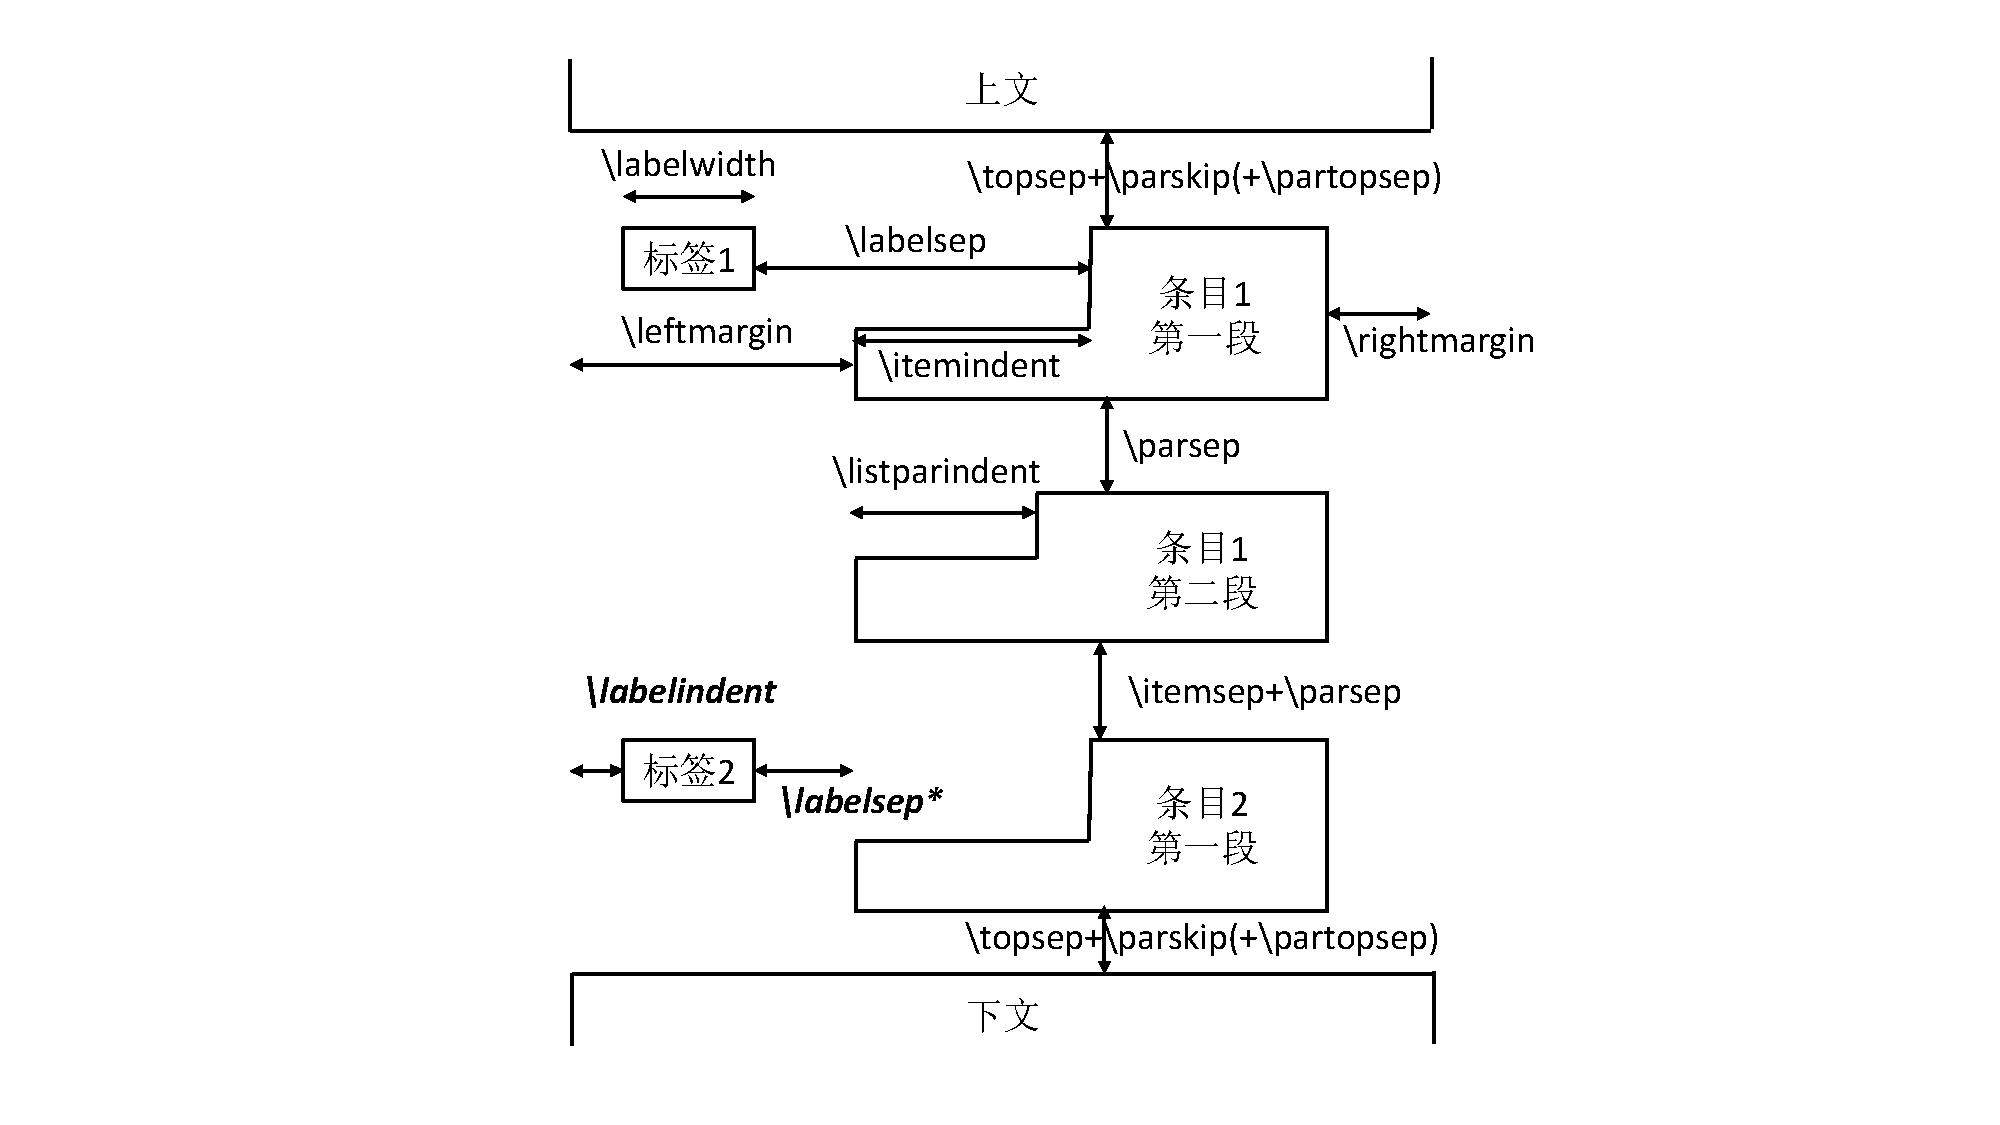
\includegraphics[width=0.9\linewidth]{enumitemsep.pdf}
\caption{列表长度参数总图}
\label{fig:enumitemsep}
\end{figure}

\fref{fig:enumitemsep}中的竖直空距topsep, partopsep, parsep, itemsep,以及水平空距left/rightmargin, listparindent, labelwidth, labelsep, itemindent都是可以直接以\texttt{key=value}的形式写在列表环境后做参数的.

命令\latexline{setlist},用于定义列表环境的样式.比如可以更改原有的列表:
\begin{latex}
\setlist[enumerate]{label=\arabic* -,
    font=\bfseries, itemsep=0pt}
\setlist[itemize]{label=$\bullet$,
    font=\bfseries,leftmargin=\parindent}
\setlist[description]{font=\bfseries\uline}
\end{latex}

最后,说一下行内列表.在加载\pkg{enumitem}宏包时使用inline选项即可启用,环境名是\envi{enumerate*}. 参数有:
\begin{para}
\item[before] 在行内列表插入前的文本,一般是冒号.
\item[itemjoin] 各\latexline{item}之间的文本,一般是逗号或者分号.
\item[itemjoin*] 倒数第二个与最后一个\latexline{item}间的文本,一般是``, and''或者“,还有”之类.
\end{para}

几个小例子.\envi{description}环境:

\begin{codeshow}
\begin{description}
[font=\bfseries\uline]
    \item[This]is BFSERIES.
    \item[And]this also.
\end{description}
\end{codeshow}

编号数字左端与左页边平齐:
\begin{latex}
\begin{enumerate}[leftmargin=*]
\end{latex}

\noindent\begin{boxedminipage}{\linewidth}
\setlength{\parindent}{2em}
Here we go. This is a very long sentence and you will find that it goes to the second line in order to show how long its parindent is.
\begin{enumerate}[leftmargin=*]
\item The left sides
\item of the label number
\item have equal indent with
\item the text parindent.
\end{enumerate}
\end{boxedminipage}
\dpar

编号数字左端与段首缩进位置平齐:
\begin{latex}
\begin{enumerate}[labelindent=\parindent,leftmargin=*]
\end{latex}

\noindent\begin{boxedminipage}{\textwidth}
\setlength{\parindent}{2em}
Here we go. This is a very long sentence and you will find that it goes to the second line in order to show how long its parindent is.
\begin{enumerate}[labelindent=\parindent,leftmargin=*]
\item The left sides
\item of the label number
\item have equal indent with
\item the text parindent.
\end{enumerate}
\end{boxedminipage}
\dpar

编号项目正文与段首缩进位置平齐:
\begin{latex}
\begin{enumerate}[leftmargin=\parindent,start=3]
\end{latex}

\noindent\begin{boxedminipage}{\textwidth}
\setlength{\parindent}{2em}
Here we go. This is a very long sentence and you will find that it goes to the second line in order to show how long its parindent is.
\begin{enumerate}[leftmargin=\parindent,start=3,]
\item An item can be extremely long. You cannot know how its parindent works if it is too short to reach the second line.
\item This is short.
\end{enumerate}
\end{boxedminipage}
\dpar

标签加框:
\begin{latex}
\begin{enumerate}[label=\fbox{\Roman*},labelindent=\parindent]
\end{latex}

\noindent\begin{boxedminipage}{\textwidth}
\setlength{\parindent}{2em}
Here we go. This is a very long sentence and you will find that it goes to the second line in order to show how long its parindent is.
\begin{enumerate}[label=\fbox{\Roman*},labelindent=\parindent]
\item An item can be extremely long. You cannot know how its parindent works if it is too short to reach the second line.
\item This is short.
\end{enumerate}
\end{boxedminipage}
\dpar

最后,本手册使用了如下5种:
\begin{latex}
\begin{description}[font=\bfseries\uline,labelindent=\parindent,
    itemsep=0pt,parsep=0pt,topsep=0pt,partopsep=0pt]
\begin{description}[font=\bfseries\ttfamily,itemsep=0pt,
    parsep=0pt,topsep=0pt,partopsep=0pt]
\begin{enumerate}[font=\bfseries,labelindent=0pt,itemsep=0pt,
    parsep=0pt,topsep=0pt,partopsep=0pt]
\begin{itemize}[font=\bfseries,itemsep=0pt,parsep=0pt,
    topsep=0pt,partopsep=0pt]
% 行内列表定义
\newenvironment{inlinee}
    {\begin{enumerate*}[label=(\arabic*), font=\rmfamily,
    before=\unskip{:}, itemjoin={{;}}, itemjoin*={{,以及:}}]}
    {\end{enumerate*}.}
\end{latex}

\section{\bibtex\ / \biber\ 参考文献}
\label{sec:bibtex}

首先说一下基础的使用.通过重定义\latexline{refname}或\latexline{bibname},前者是article类,后者是book类.这点在\secref{subsec:cite}这一节已经介绍过.

关于怎样将参考文献正常编号并加入目录中,请参考\secref{subsec:cite}这一节.

\begin{latex}
\renewcommand{\bibname}{参考文献}
\end{latex}

在文献目录之前、文献标题之下,用\latexline{bibpreamble}插入一段文字:
\begin{latex}
\renewcommand{\bibpreamble}{以下是参考文献:}
\end{latex}

用\latexline{bibfont}更改参考文献的字体:
\begin{latex}
\renewcommand{\bibfont}{\small}
\end{latex}

用\latexline{citenumfont}定义在正文中引用时,文献编号的字体:
\begin{latex}
\renewcommand{\citenumfont}{\itshape}
\end{latex}

用\latexline{bibnumfmt}定义文献目录的编号,默认是[1], \ldots 形式.比如改成加点形式:
\begin{latex}
\renewcommand{\bibnumfmt}[1]{\textbf{#1.}}
\end{latex}

文献项之间的间距更改,调整\latexline{bibsep}即可:
\begin{latex}
\setlength{\bibsep}{1ex}
\end{latex}

\subsection{\texttt{natbib}宏包}
个人认为文献宏包首推\pkg{natbib},不再推荐\pkg{cite}. \pkg{natbib}宏包的加载选项:
\begin{para}
\item[round] (默认)圆括号.
\item[square/curly/angle] 方括号/花括号/尖括号.
\item[semicolon/comma] 分号/逗号作为文献序号分隔符.
\item[authoryear] “作者+年代(AuY)”模式显示参考文献.
\item[numbers] “数字编号(num)”模式显示参考文献.
\item[super] 参考文献显示在上标.
\item[sort(\&compress)] 排序文献序号(并压缩\footnote{压缩是指:连续三个或以上的序号会显示为如2--4的形式.}).
\item[compress] 压缩但不排序.
\item[longnamefirst] 长名称在前,缩写名称在后.
\item[nonamebreak] 防止作者名称中间出现断行.可能造成Overfull坏箱,但能解决某些hyperref异常.
\item[merge] 允许*形式的引用.
\item[elide] 在merge选项引用中,省略相同的作者或年份.
\end{para}

你也可以通过宏包提供的\latexline{setcitestyle}命令:
\begin{feae}
\item 引用模式:authoryear, number与super三种,含义同上.
\item 引用分隔符:semicolon, comma, 或者用citesep=\{\textit{sep}\}来指定.
\item 作者与年代间的符号:aysep=\{\textit{sep}\}
\item 同作者下多个年代间的符号:yysep=\{\textit{sep}\}
\item 说明文字后的符号:notesep=\{\textit{sep}\}
\end{feae}

默认的参数是:
\begin{latex}
\setcitestyle{authoryear,round,comma,aysep={;},
    yysep={,},notesep={, }}
\end{latex}

除了\LaTeX\ 原生的\latexline{cite}命令,\pkg{natbib}宏包还提供了\tref{tab:natbib}所示的引用命令.

\begin{table}[!hbt]
\centering
\caption{\texttt{natbib}宏包命令表}
\label{tab:natbib}
\small
\begin{tabular}{l|>{\ttfamily}l!{$\Rightarrow$}l}
\hline
\multicolumn{3}{c}{使用\latexline{Citet}, \latexline{Citep}, \latexline{Citealt}, \latexline{Citealp}确保姓名首字母大写} \\
\hline
\multicolumn{3}{l}{\latexline{citet} \& \latexline{citet*}} \\
\hline
\multirow{4}*{AuY}
& citet\{jon90\} & Jones et al. (1990) \\
& citet[chap.2]\{jon90\} & Jones et al. (1990, chap.2) \\
& citet\{jon90, jam91\} & Jones et al. (1990); James et al. (1991) \\
& citet*\{jon90\} & Jones, Baker, and Williams (1990) \\
\cline{2-3}
\multirow{2}*{num}
& citet\{jon90\} & Jones et al. [21] \\
& citet[chap.2]\{jon90\} & Jones et al. [21, chap.2] \\
\hline

\multicolumn{3}{l}{\latexline{citep} \& \latexline{citep*}} \\
\hline
\multirow{6}*{AuY}
& citep\{jon90\} & (Jones et al., 1990) \\
& citep[chap.2]\{jon90\} & (Jones et al., 1990, chap.2) \\
& citep[see][]\{jon90\} & (see Jones et al., 1990)\\
& citep[see][chap.2]\{jon90\} & (see Jones et al., 1990, chap.2)\\
& citep\{jon90, jon91\} & (Jones et al., 1990, 1991) \\
& citep*\{jon90\} & (Jones, Baker, and Williams, 1990) \\
\cline{2-3}
\multirow{5}*{num}
& citep\{jon90\} & [21] \\
& citep[chap.2]\{jon90\} & [21, chap.2] \\
& citep[see][]\{jon90\} & [see 21] \\
& citep[see][chap.2]\{jon90\} & [see 21, chap.2]\\
& citep{jon90a,jon90b} & [21, 32] \\
\hline

\multicolumn{3}{l}{\latexline{cite}} \\
\hline
AuY & \multicolumn{2}{c}{此模式下与\latexline{citet}相同} \\
\cline{2-3}
num & \multicolumn{2}{c}{此模式下与\latexline{citep}相同} \\
\hline\hline

\multicolumn{3}{l}{\latexline{citealt}: 与\latexline{citet}相似,但没有括号.} \\
\hline
\multicolumn{3}{l}{\latexline{citealp}: 与\latexline{citep}相似,但没有括号.} \\
\hline
\multicolumn{3}{l}{\latexline{citenum}: 引用文献编号.} \\
\hline
\multicolumn{3}{l}{\latexline{citetext}: 打印一段文本.} \\
\hline
\multicolumn{3}{l}{\latexline{citeauthor} \& \latexline{citeauthor*}: 引用文献的作者.带星表示显示该文献的全部作者.} \\
\hline
\multicolumn{3}{l}{\latexline{citeyear} \& \latexline{citeyearpar}: 引用文献的年份.par的意思是在文献外加括号.} \\
\hline
\end{tabular}
\end{table}

\subsection{\bibtex 使用}
\bibtex 通过单独的.bib扩展名文件管理文献,使多文档方便地共用一份文献列表(可以指引用其中的部分文献)成为可能.使用时请确保:
\begin{feae}
\item 确保你的文档定义了\latexline{bibliographystyle}类型.\LaTeX\ 预定义的类型分为:
  \begin{para}
    \item[plain] 按照第一作者字母顺序排序.“\textit{作者. 文献名. 出版商或刊物, 出版地, 出版时间.} ”
    \item[unsrt] 按引用顺序排序.
    \item[alpha] 按作者名称和出版年份排序.
    \item[abbrv] 缩写形式.
  \end{para}
\item 在文档中插入了\latexline{cite}等命令.
\item 在参考文献列表位置插入了\latexline{bibliography}命令\footnote{如果你在正文中使用\latexline{nocite\{ref-name\}}命令,可以把bib文件中未cite的文献也加入到列表.想全部加入,在正文中使用\latexline{nocite\{*\}}命令.}.
\end{feae}

一个通用的\bibtex\ 使用方式:
\begin{latex}
\bibliographystyle{plain}
\begin{document}
    ...
    ... and published here\cite{Smith93TRB}.
    ...
    \bibliography{myBib}
\end{document}
\end{latex}

然后在你的myBib.bib文件中,你需要有类似这样的条目.等号后使用花括号或引号均可.
\begin{latex}
% 如果引用期刊
@article{Smith1993TRB,
    author = {作者, 多个作者用and 连接},
    title = {标题},
    journal = {期刊名},
    number = {页码},
    year = {年份}}
% 如果引用书籍
@book{Smith1993TRB,
    author ="作者",
    year="年份2008",
    title="书名",
    publisher ="出版社名称"}
\end{latex}

一些其他的注意事项:
\begin{feai}
  \item \textbf{通常你无须手动书写 bib 内容}。许多文献检索页面(比如 Google 学术)都支持导出\bibtex 文本,将其粘贴到你的 \texttt{.bib} 文件中即可.
  \item 除了上例介绍的文献类型.更多的文献类型以及它们的使用条目选项,参考\tref{tab:bibtype}.一个可能用到的场景是引用网页,但它并没有专门的类型。作为参考,我一般用\texttt{misc}类型,并在其\texttt{note}键中标出访问时间。
  \item 等号后的花括号表示直接输出,不通过 \bibtex 自动转换大小写。这常用于强制字母大小写的场合,比如\texttt{title=\{UpperCaseVar\}}。
\end{feai}

\begin{table}[!htb]
\centering
\caption{\bibtex 文献类型常用表}
\label{tab:bibtype}
\begin{tabular}{>{\ttfamily}ll}
\hline
article & 期刊文献 \\
& 必要:author, title, journal, year \\
& 选填:volume, number, pages, month, note \\
\hline
book & 公开出版图书 \\
& 必要:author/editor, title, publisher, year \\
& 选填:volume/number, series, address, edition, month, note \\
\hline
booklet & 无出版商或作者的图书.必要:title\\
& 选填:author, howpublished, address, month, year, note \\
\hline
conference/ & 无出版商或作者的图书.必要:title \\
inproceedings & 选填:author, howpublished, address, month, year, note \\
\hline
incollection & 书籍含独立标题的章节,比如论文集的一篇 \\
& 必要:author, title, booktitle, publisher, year \\
& 选填:editor, volume/number, series, type, chapter, pages, \\
& address, edition, month, note \\
\hline
manual & 技术手册.必要:title \\
& 选填:author, organization, address, edition, month, year, note \\
\hline
mastersthesis & 硕士论文\\
& 必要:author, title, school, year \\
& 选填:type, address, month, note\\
\hline
misc & 其他 \\
& 选填:author, title, howpublished, month, year, note \\
\hline
phdthesis & 博士论文 \\
& 必要:author, title, year, school\\
& 选填:address, month, keywords, note\\
\hline
techreport & 教育,商业机构的技术报告\\
& 必要:author, title, institution, year\\
& 选填:type, number, address, month, note\\
\hline
unpublished & 未出版的论文或图书\\
& 必要:author, title, note\\
& 选填:month, year\\
\hline
\end{tabular}
\end{table}

最后,你可能需要\RED{编译\xelatex , 再编译\bibtex , 最后连续编译两次\xelatex 来完成你的文档建立}.

\section{索引}
使用\pkg{makeidx}宏包来建立索引.索引标题通过重定义\latexline{indexname}更改.
\begin{feae}
\item 在导言区加载\pkg{makeidx}宏包,并输入\latexline{makeindex}开始收集索引.
\item 在文中使用\latexline{index}命令来插入索引标签.
\item 在需要插入索引列表的位置输入\latexline{printindex}.
\end{feae}

索引命令\latexline{index}的用法如\tref{tab:index}.注意:这四种符号\verb+!|@"+如果要写在参数中,请在它们之前添加一个双引号.
\begin{table}
\centering
\tabcaption{索引命令\texttt{\char92 index}的使用}
\label{tab:index}
\begin{tabular}{>{\ttfamily}ll}
\hline
\multicolumn{1}{l}{\textbf{例子}} & \textbf{效果} \\
\hline
\multicolumn{2}{l}{!: 分级索引,最多三级} \\
hello & hello, 1 \\
hello!Foo & \hspace{1em}Foo, 2 \\
hello!Foo!bar & \hspace{2em}bar, 3 \\
\hline
\multicolumn{2}{l}{@: 格式化,“排序字串@显示样式”}\\
alpha@\$\char92 alpha\$ & $\alpha$, 4 \\
BOLD@\char92 textbf\{BOLD\} & \textbf{BOLD}, 5 \\
\hline
\multicolumn{2}{l}{|: 页码显示}\\
wow|( & \multirow{2}*{wow, 6--13} \\
wow|) & \\ 
Meow|textbf & Meow, \textbf{14} \\
Meow|see\{hello\} & Meow, \textit{see} hello \\
Meow|seealso\{wow\} & Meow, \textit{see also} wow \\
\hline	
\end{tabular}
\end{table}

此外,\pkg{imakeidx}宏包可能更强,它允许索引分组:
\begin{latex}
\makeindex[title={Group 1}]
\makeindex[title={Group 2},name=another]
% 以上在导言区,且需要\usepackage{imakeidx}
    ...\index{...}
    ...\index[another]{...}
\printindex
\printindex[another]
\end{latex}

定制索引样式可使用\pkg{imakeidx}宏包;另一个宏包\pkg{idxlayout}也能实现这些功能,不过需要放置在前者之后加载.

使用 \pkg{tocbibind} 宏包将索引章节正常编号或编入目录项,参考\secref{pkg:tocbibind}部分.

关于索引,部分用户有制作词汇表的需求,请参考\pkg{glossary}宏包.

\section{公式与图表编号样式}
\subsection{取消公式编号}
取消单行公式的编号,用\latexline{[\char`\\]}或者\envi{equation*}环境,代替\envi{equation}环境.

取消多行公式中某行的编号,使用\pkg{amsmath}宏包的\latexline{notag}或\latexline{nonumber}命令.命令放在对应行的末尾即可.该方法同样适用于\envi{equation}环境.

取消多行公式中所有行的编号,请使用\envi{align*}环境而不是\envi{align}环境.你可以参考\secref{subsec:multieqnum}内容.

\subsection{增加公式编号}
\pkg{amsmath}宏包提供了增加编号的\latexline{tag}命令:

\begin{codeshow}
\[a^2>0 \tag{$\star$}\]
\begin{equation}
b^2 \geqslant 0
\tag*{[Axiom]}
\end{equation}
\end{codeshow}

其中\latexline{tag*}命令会去掉编号行间公式的小括号,从而定制性更强.如果想在\RED{多行公式中的某行}添加编号,使用\latexline{numberthis}命令.

\subsection{父子编号:公式1与公式1a}
有时你需要叙述一些推论,你不希望这些推论被编号为公式,但是不进行编号又难以叙述.这时可以尝试\pkg{amsmath}宏包提供的\envi{subequations}环境:

\begin{codeshow}
\begin{subequations}
This is an upright text.
\begin{align}
A' &=B+C \\
X &=0 \nonumber \\
D' &=E \times F
\end{align}
Enjoy this environment.
\end{subequations}
\end{codeshow}

父子编号样式的定义参考\hyperref[code:parenteqnum]{这里}.还有一种利用计数器的方式,可以插入公式1和公式1'这样的效果,但是实现起来稍显麻烦.参考\hyperref[code:eq1plus]{这里}.

\subsection{在新一节重新编号公式}
只需要\latexline{numberwithin}进行设置:
\begin{latex}
\numberwithin{equation}{section}
\end{latex}

对于article文档类,显示为(2.1), (2.2), \ldots ;对于chapter等文档类,显示为(1.2.1), (1.2.2), \ldots 这样.

\subsection{公式编号样式定义}
通过控制计数器的方式可以方便地自定义公式编号样式:
\begin{latex}
% 更改为:(2-i), (2-ii)
\renewcommand{\theequation}{\thechapter-\roman{equation}}
% 父子公式编号样式,在subequation环境内使用
% 效果:(4.1-i), (4.1-ii)
\renewcommand{\theequation}`\label{code:parenteqnum}`
    {\theparentequation-\roman{equation}}
\end{latex}

公式1和公式1'的实现方法可以这样:\label{code:eq1plus}
\begin{latex}
\begin{equation}\label{eq:example}
    A=B,\ B=C
% 需要标记的公式内部给myeq计数器赋值
\setcounter{myeq}{\value{equation}}
\end{equation}
插入另一个式子:
\begin{equation}
    D>0
\end{equation}
由式\ref{eq:example}可以推出式\ref{eq:example'}:
\begin{equation}\label{eq:example'}
    \tag{\arabic{chapter}.\arabic{myeq}$'$}
    A=C
\end{equation}
\end{latex}

\section{附录}
\label{sec:appendix}
附录可以直接在文中需要开启的地方,使用下述命令.此后的最高大纲级别编号会变为大写英文字母:A, B, C, \ldots
\begin{latex}
\appendix
\end{latex}

你也可以使用\pkg{appendix}宏包.加载时常用的选项:
\begin{para}
\item[titletoc:] 目录中显示为``Appendix A''而不是只有一个``A''.如果你不喜欢Appendix这个名称,用重定义\latexline{appendixname}命令即可.
\item[header:] 在附录页的标题前插入同样的名称.
\end{para}

附录一般出现在\envi{document}环境内部的最后,例如:
\begin{latex}
% 导言区:\usepackage[titletoc]{appendix}
\begin{appendices}
\renewcommand{\thechapter}{\Alph{chapter}}
\titleformat{\chapter}[display]{\Huge\bfseries}
    {附录\Alph{chapter}}{1em}{}
\chapter{...} ...
\end{appendices}
\end{latex}

本手册使用的是\latexline{appendix}命令,并在其后重定义了chapter的显示样式.读者可以从源码中参考.

\section{自定义浮动体*}
可以使用\pkg{newfloat}宏包自定义浮动体.形如:
\begin{latex}
\DeclareFloatingEnvironment[`\textit{options}`]{`\textit{float-name}`}
\end{latex}

选项包括:
\begin{para}
\item[name] 标签内容.如name=插图.
\item[listname] 目录名.如listname=插图目录.
\item[fileext] 目录文件扩展名,默认是\textit{float-name}前加lo.
\item[placement] 位置参数htbp.
\item[within] 父计数器名称.比如chapter. 可以设为none.
\item[chapterlistsgaps] 赋值on/off. 是否允许浮动体目录中,不同章节的浮动体间有额外的空距.
\end{para}

要输出浮动体目录,请插入命令\latexline{listof[float-name]s}.

\section{编程代码与行号*}
\label{sec:coding}
\subsection{\texttt{listings}宏包}
编程代码不是用\envi{verbatim}环境输出的……\pkg{listings}宏包是个好选择.你可以打开它的宏包文档查看它支持的编程语言,包括C/C++, Python, Java等等.当然还有\LaTeX,如果它也算编程代码的话.你也可以自定义一个全新的语言.预定义或自定义的语言均可用\latexline{lstset}命令来设置.
\begin{latex}
\lstdefinelanguage{`\textit{languagename}`}{`\textit{key=value}`}
% 设置
\lstset{language=`\textit{languagename}`, `\textit{key=value}`}
\end{latex}

可调整的参数包括:
\begin{para}
\item[language] 用于\latexline{lstset}中,表示设置只对该语言生效.该参数有可选参数,比如[Sharp]C表示C\#,具体需要查看listings宏包.
\item[basicstyle] 基础输出格式,一般是\latexline{small\char`\\ttfamily}
\item[commentstyle] 注释样式.
\item[keywordstyle] 保留词样式.
\item[sensitive] 保留词是否大小写敏感.默认false,可选true/false.
\item[stringstyle] 字符串样式.
\item[showstringspaces] 显示字符串中的空格.
\item[numbers] 行号样式,默认是none. 可选left/right.
\item[stepnumber] 默认是1,即每行都显示行号.
\item[numberfirstline] 默认false,即如果stepnumber$>1$,首行不显示数字.
\item[numberstyle] 行号样式.
\item[numberblanklines] 默认true,即在空白的代码行也显示行号.
\item[firstnumber] 默认auto,可选last或填入数字,表示起始行号.
\item[frame] 默认single,即trbl,分别表示top, right, buttom, left四条边的线都是单线.如果想变某边为双线,大写它:trBL.
\item[frameround] 在\latexline{lstset}中,从右上角顺时针设置,代码框为直角或圆角.比如fttt表示仅右上为直角.
\item[framerule] 代码框的线宽.
\item[backgroundcolor] 定义frame里代码的背景色,如\latexline{color\{red\}}.
\item[belowskip] 默认\latexline{medskipamount}.代码框下端到下文正文的竖直距离.
\item[aboveskip] 类似.
\item[columns] 设置行内单词间距的处理方式.fixed 选项会强行按列对齐,可能产生字母覆盖问题;space-flexible 选项会调整现有空距尝试对齐列;flexible 选项可能在原本无空距的地方插入空距来尝试对齐;而 fullflexible 选项(本文使用)则完全不管列对齐.
\item[emptylines] 设置最多允许的空行,比如=1,会使多于1行的空行全部删除,并不计入行号.如果写为=*1,被删除的行的行号仍然会保留计数.
\item[esacpeinside] 暂时脱离代码环境而输入一些\LaTeX\ 支持的命令,比如临时输入斜体.一般设置为一对重音符号(键盘数字1左侧的符号).
\end{para}

代码环境的调用方式是\envi{lstlisting}环境,例如:
\begin{latex}
\begin{lstlisting}[language=Python]
for loopnum in lst:
    sum += lst[loopnum]
\end{lstlisting}
\end{latex}

也可以利用\latexline{lstnewenvironment}命令定义一个代码输出环境:
\begin{latex}
\lstnewenvironment{`\textit{envi-name}`}
    [`\textit{opt}`][`\textit{opt default}`]
    {`\textit{before-code}`}{`\textit{after-code}`}
% 调用:
\begin{envi-name}...\end{envi-name}
\end{latex}

如果只想在行内输出,可以像这样用\latexline{lstinline}定义:
\begin{latex}
\newcommand{\inlatexline}[1]{{\lstinline
    [language=TeX,basicstyle=\small\ttfamily]{#1}}}
% 要防止“#include”双写“#”,请调用 xparse 宏包:
\NewDocumentCommand{\cppline}{v}{{\lstinline
    [language=C++]{#1}}}
\end{latex}

有时候,一些关键词并没有被宏包成功高亮,或者你需要更多种类的高亮方式,这时候你可以自己设置:
\begin{latex}
\lstset{language=..., classoffset=0,
    morekeywords={begin,end},
    keywordstyle=\color{brown},
    classoffset=1,...}
\end{latex}

除了morekeywords外,你可以使用:
\begin{latex}
\lstdefinestyle{...}{
    morecomment=[l]{//}, % 单行注释
    morecomment=[s]{/*}{*/}, % 多行注释,不可嵌套
    morecomment=[n]{(*}{*)}, % 多行注释,可嵌套
    morestring=[b]", % 字符串
% 如果想在字符串内输出该符,前加反斜杠即可
\end{latex}

代码环境在复制的时候怎么才能不复制前面的行号呢?在导言区加上,
\begin{latex}
\usepackage{accsupp}
\newcommand{\emptyaccsupp}[1]
    {\BeginAccSupp{ActualText={}}#1\EndAccSupp{}}
% 在lstset的numberstyle中加入
...numberstyle=...\emptyaccsupp...,
\end{latex}

\RED{并请用Adobe Reader等功能健全的PDF阅读打开pdf}!如果是Sumatra仍然可能会选中前面的行号.

最后,给出本手册旧版中使用的\LaTeX\ 的\latexline{lstset},颜色另行定义:
\begin{latex}
% \emptyaccsupp 来自前文利用宏包 accsupp 的自定义
\lstset{language=[LaTeX]TeX,
    basicstyle=\small\ttfamily,
    commentstyle=\color{commentcolor},
    keywordstyle=\color{keywordcolor},
    stringstyle=\color{stringcolor},
    showstringspaces=false,
    % Package/Tikz-Lib Using
    classoffset=0,
    morekeywords={begin,end,usetikzlibrary},
    keywordstyle=\color{keywordcolor},
    classoffset=1,
    morekeywords={article,report,book,xeCJK,tikz,calc},
    keywordstyle=\color{packagecolor},
    classoffset=2,
    morekeywords={document,tikzpicture},
    keywordstyle=\color{envicolor},
    % Line Number Style
    numbers=left,stepnumber=1,
    numberstyle=\tiny\emptyaccsupp,    
    % Frame and Background Color
    frame=single,framerule=0pt,    
    backgroundcolor=\color{backcolor},
    % Spaces
    emptylines=1,escapeinside=`\texttt{\char96{}\char96{}}`}
\end{latex}

\subsection{\texttt{tcolorbox}宏包}
\label{subsec:tcolorbox}
本手册在修订过程中发现了一个可以方便地“一侧写源代码,另一侧展示结果”的宏包,名叫\pkg{tcolorbox};因此基本用其替换了原有的\pkg{listings}宏包——但是引擎仍然使用的是\pkg{listings},在使用新宏包时也需要借助旧宏包选项来设置引擎.

该宏包支持下,本手册旧版使用的\latexline{newtcblisting}定义了\LaTeX\ 代码环境:
\begin{latex}
\usepackage{tcolorbox}
  \tcbuselibrary{listings,skins,breakable}
% listings是代码展示引擎,breakable为了可跨页
\newtcblisting{latex}{breakable,skin=bicolor,colback=gray!30!white,
  colbacklower=white,colframe=cyan!75!black,listing only, 
  left=6mm,top=2pt,bottom=2pt,fontupper=\small,
  % listing style
  listing options={style=tcblatex,
  keywordstyle=\color{blue},commentstyle=\color{green!50!black},
  numbers=left,numberstyle=\tiny\color{red!75!black}\emptyaccsupp,
  emptylines=1,escapeinside=``}}
\end{latex}

其中很多选项意义显然,就不赘述了.需要指明的有:
\begin{para}
\item[skin] bicolor,让源代码和显示结果可以分开设置背景色.
\item[colbacklower] 背景色.\texttt{tcolorbox}分为两段,下段(或右段)叫lower.
\item[fontupper] 上段(或左段)叫upper,这是设置在进入upper前插入的格式命令,不局限于字号.
\item[代码展示参数] 该参数经常用到的是:
    \begin{para}
      \item[listing only] 仅展示源代码.也有text only选项.
      \item[listing and text] 上段源代码,下段结果.本手册的\envi{codeshowabove}环境采用该参数.如果text与listing交换,即上段结果下段源代码.
      \item[listing side text] 左段源代码,右段结果.本手册的\envi{codeshow}环境就采用了该参数.同样也可以交换,变成左段结果右段源代码.
      \item[listing outside text] 同上,只是结果“看起来”在盒子外.
    \end{para}
\item[listing option] 除了特殊的style字段,这些参数都会被传递给引擎(本手册是listings宏包).\texttt{style=tcblatex}是\pkg{tcolorbox}宏包预定义的.
\end{para}

该环境也支持使用可选参数,用法类似原生 \latexline{newcommand} 命令.但是,如果你只有一个参数,而且它是可选的,请使用 \latexline{NewTCBListing} 命令(需要用 \latexline{tcbuselibrary} 命令 加载 \texttt{xparse} 库)以避免可能的问题。例如,利用如下命令\footnote{\TeX\ Live 2019版的宏包目前存在一个问题,在定义单个参数且其为可选参数时,需要在字母O前添加感叹号。}可以定义一个左侧源码、右侧排版结果的展示环境:
\begin{latex}
% 调用可无参或单参,例:\begin{codeshow}
% 或 \begin{codeshow}[listing and text]
\NewTCBListing{codeshow}{ !O{listing side text} }{
  skin=bicolor,colback=gray!30!white,
  colbacklower=pink!50!yellow,colframe=cyan!75!black,
  valign lower=center,
  left=6mm,righthand width=0.4\linewidth,fontupper=\small,
  % listing style
  listing options={style=latexcn},#1
}
\end{latex}
其中,\texttt{O} 这种用法请参考 \pkg{xparse} 宏包文档,常用的有必选参数“m”、可选参数“o”、可选参数并指定缺省值“O\{<default>\}”.

通过该宏包的\latexline{newtcbox}命令,本手册实现了对于命令、环境、宏包的高亮.以下给出本手册中对宏包名称的高亮作为例子,参数含义显然:
\begin{latex}
\newtcbox{\pkg}[1][orange!70!red]{on line,
    before upper={\rule[-0.2ex]{0pt}{1ex}\ttfamily},
    arc=0.8ex,colback=#1!30!white,colframe=#1!50!black,
    boxsep=0pt,left=1.5pt,right=1.5pt,top=1pt,bottom=1pt,    boxrule=1pt}
\end{latex}

实际上\pkg{tcolorbox}的强大之处远不止此,它能做出颜值很高的箱子样式.更多的内容请自行查阅其宏包文档学习.最后,附上\pkg{tcolorbox}预定义的 \texttt{tcblatex} 的 \texttt{style}选项\footnote{该定义位于\texttt{texmf-dist/tex/latex/tcolorbox/tchlistings.code.tex}中.},是用 \TeX\ 编写的,读者可以与本手册源码中的定义进行对比:
\begin{latex}
\lstdefinestyle{tcblatex}{language={[LaTeX]TeX},
     aboveskip={0\p@ \@plus 6\p@}, belowskip={0\p@ \@plus 6\p@},
     columns=fullflexible, keepspaces=true,
     breaklines=true, breakatwhitespace=true,
     basicstyle=\ttfamily\small, extendedchars=true, nolol,
     inputencoding=\kvtcb@listingencoding}
\end{latex}


\subsection{行号}
\begin{linenumbers}
\modulolinenumbers[3]
行号使用\pkg{lineno}宏包进行生成,在此简单介绍宏包选项:
\begin{para}
  \item[left]默认选项,行号出现在左页边.
  \item[right]右页边.
  \item[switch]对于双页排版的文档,偶数页左页边,奇数页右页边.
  \item[switch*]对于双页排版的文档,置于内侧页边.
  \item[running]默认选项.整个文档进行计数.
  \item[pagewise]每页行号重新从1计数.
  \item[modulo]每5行显示行号.
  \item[displaymath]自动将\LaTeX\ 默认行间公式放在新定义的\envi{linenomath}环境中.
  \item[mathline]如果使用了\envi{linenomath}环境,则对其中的数学公式也编行号.
\end{para}

如果你想开始编号,使用\latexline{linenumbers[number]}命令,其中\textit{number}表示起始行号;并用\latexline{nolinenumbers}来结束.或者选择使用\envi{(running)linenumbers}环境,并且仿上设置起始行号.如果使用\latexline{linenumbers*}, \latexline{runninglinenumbers}或者\envi{linenumbers*}、\envi{runninglinenumbers*}环境,那么行号会自动从1开始.

你可以使用\latexline{resetlinenumber[number]},在某处把行号设置为某个数值.

如果想要每N行显示行号,使用\latexline{modulolinenumbers[N]}命令.比如:
\end{linenumbers}

\begin{latex}
\begin{linenumbers}
    \modulolinenumbers[3]
    ...TEXT...
\end{linenumbers}
\end{latex}

本节的subsection后到代码段前的所有内容就是包含在如上的环境中的.